% Software Requirements
% CS 461 - CS Senior Capstone
% Fall 2017
% Authors: Connor Christensen, Lily Shellhammer, William Buffum


\documentclass[draftclsnofoot,onecolumn,letterpaper,10pt,compsoc]{IEEEtran}

% Packaging
\usepackage{geometry}
\usepackage{hyperref}
\usepackage{titling}
\usepackage{color}
\usepackage{listings}
\usepackage{cite}
\usepackage{pdfpages}

% Paper type
\geometry{letterpaper, margin=.75in}

% Title page
\title{CS 461 - CS Senior Capstone
	\\Fall 2017
	\\Problem Statement
}


\author{
	Connor I. Christensen \\
	\texttt{chriconn@oregonstate.edu}
	\\
	Lily M. Shellhammer \\
	\texttt{shellhal@oregonstate.edu}
	\\
	William B. Buffum \\
	\texttt{buffumw@oregonstate.edu}
}

\begin{document}

\begin{titlingpage}
    \maketitle
    \begin{abstract}
			Ninkasi Brewing Company is using an outdated brewing operations management system. To update the data management system, the BrewHops team will implement a web application and relational database.
			\\
			\textbf{Keywords:} Brewing, Operations, Management, Ninkasi
    \end{abstract}
		\pagebreak
		\tableofcontents
\end{titlingpage}

\section{Introduction}
	\subsection{Purpose}
    In this document, we outline the requirements for Ninkasi’s brewing operations data management system we will implement. This includes a detailed description of the product created and the technology we will be using to complete the product. This document is intended for a technical audience and will be used primarily by our instructors, Kirsten Winters and Kevin McGrath, and our sponsor, Daniel Sharp.
    
	\subsection{Scope}
    We will develop a web application and relational database model to manage Ninkasi data. We will perform a cost-benefit analysis to recommend hosting system with web service provider versus hosting on Ninkasi servers. Database will store: beer type identifier, batch number, GEN\footnote{Need clarification from Daniel on what this is}, Dry Hop/Adjunct Type\footnote{Need clarification from Daniel on what this is}, hop amount, and data on internal brewing vat (IBV) measurements. IBV data points include: S.G.\footnote{Need clarification from Daniel on what this is}, pH level, Alcohol By Volume (ABV), and beer temperature. Provided interface will allow brewers to manually insert new batch records, update incorrect data, and view existing data. Interface will allow Ninkasi personnel to view data using downloadable .csv files. We will gage adequacy of interface based on 60\% approval from Ninkasi personnel, of which Daniel Sharp must approve. The goal of these requirements is to stop paper tracking of information and stop use of Excel as primary data storage.
    \\
    \\
    Stretch goals include: login system and data viewing in browser (no download required).
    \\
    \\
    We are not be responsible for application security, data integrity (during manual entry), or direct control of any brewing process.
    
	\subsection{Definitions, acronyms and abbreviations}
    Data collected by our database will be referred to as “cellaring data”. This means data that has been collected while cellaring beers. Data points include but are not limited to: beer temperature, maturation time, amount of hops and other materials added. 
    
	\subsection{References}
    No references as of 10/27/2017.
	\subsection{Overview}
    In the next sections, this document outlines details on the hardware, software, and user interface requirements for our project. It explains what needs to be done in order to launch our minimum viable product. Security, functionality, and organization are explained in detail.

\section{Description}
	\subsection{Product Perspective}
		\subsubsection{System interfaces}
        Brewers will interact with our web app in the cellar. The web app interacts with the database and will enter data points from the brewer's entry into the form. If we meet our stretch goals, brewers will be able to extract Excel spreadsheets from our web app.
        
		\subsubsection{User interfaces}
        The user will interact with the web app through either an internet connected phone, tablet, desktop or laptop computer. Phones will operate almost exclusively in portrait mode. Apart from the occasional chart or data display, most of the use for the phone will be entering data, which benefits from a portrait layout. Tablets have the ability to use both portrait or landscape mode, depending on how they would like to use the device, and which method is more convenient for them. Desktops and laptops will work in a landscape mode. For big enough screens, extra space can be used to fit more functionality on one page without having to hide menu items or actions, such as extracting data from the database.
        \\
        \\
        All Ninkasi brewers use a company provided phone and most of the brewer's work will be done through that phone. It's important that the site be consistent between iOS and Android to increase reliability, allow brewers to help each other with problems regardless of operating system, and reduce the learning curve. The environment in which the brewers are working requires that the data entry system be clear, easy to see and have a forgiving interface. For any new hires, the system should be intuitive\footnote{60\% acceptance of interface required to be considered "intuitive"}. Some phones may have smaller screens or may be held at a distance, so it's important that the font be big enough, the contrast strong enough, and the input boxes take up as much space as they can so they are easy to tap and input is easy to see. Brewers may have water, grain dust or other materials on their hands that will interfere with the touch capabilities of the device. Making the interface forgiving by making buttons, input fields and any other interactive components large will reduce error and frustration.
        \\
        \\
        If the system should use terminology that the brewers are familiar with. Reports should be color coded to keep the screen from filling with text and to allow the brewers to access the data at a glance.
        
		\subsubsection{Hardware interfaces}
        Ninkasi has a small server in their headquarters. A cost-benefit analysis will determine if this server will satisfy the hardware requirements of the system. If it will not, we will provide recommendations for web service providers.
        
		\subsubsection{Software interfaces}
        The user will interact with data via a web application. The application will expose input forms to submit data and downloadable .csv files to view data. We will release the software in stages, starting with a database, then a basic web input form connected to the database, then our final minimum viable product will include downloadable .csv files. 
        
		\subsubsection{Communications interfaces}
        Web application will not implement other interfaces.
        
		\subsubsection{Memory constraints}
        Currently Ninkasi has space on a single server in a back room. Ninkasi will quickly grow out of server space which would constrain how much data we can host there. If Ninkasi decides to host our database on a 3rd party cloud hosting site, the memory constraints will be those of how much space they buy.
        
		\subsubsection{Site adaptation requirements}
        Brewers will adapt to using our web form rather than continue implementing the system they previously used. They will enter data not through paper logs or emails, but only through the web app. Our web form will need to connect to the chosen database, which may be hosted on site on Ninkasi’s server.
        
	\subsection{Product functions}
    Product include development of relational database and development of web application to process and present database information. Brewers will input information to the database using a form on the website, and retrieve information from the database as a .csv file.
    
	\subsection{User characteristics}
    Brewers using the web app will have all levels of education, including PhD, MS, BS, AAS, and no college experience. Their technical expertise about web development and coding in general will be minimal, but they will understand how to use mobile applications, how to access websites, and how to enter data into forms.
    
	\subsection{Constraints}
		\subsubsection{Regulatory policies}
        Not applicable for BrewHops team.
        
		\subsubsection{Hardware limitations}
        No hardware limitations\footnote{Need to verify that BrewHops team will have access to Ninkasi server}.
        
		\subsubsection{Interfaces to other applications}
        BrewHops application will integrate with Telnet\footnote{Telnet is the system that performs physical measurements inside brewing vats} application.
        
		\subsubsection{Parallel operation}
        Database will allow concurrent read access and use transactions for insertions and updates.
        
		\subsubsection{Audit functions}
        Not applicable for BrewHops team.
        
		\subsubsection{Control functions}
        Not applicable for BrewHops team.
        
		\subsubsection{Higher-order language requirements}
        Objects and callback functionality required.
        
		\subsubsection{Signal handshake protocols (e.g., XON-XOFF, ACK-NACK)}
        Not applicable for BrewHops team.
        
		\subsubsection{Reliability requirements}
        Ensure data integrity for automated data collection. Do not ensure data integrity for manual data entry.
        
		\subsubsection{Criticality of the application}
        Application not critical to Ninkasi Brewing Company's success.
        
		\subsubsection{Safety and security considerations.}
        Not applicable for BrewHops team. BrewHops team is not ensuring proper system security.
        
	\subsection{Assumptions and dependencies}
    BrewHops team will have access to Ninkasi Brewing Company's server to deploy application.

\section{Specific requirements}
	\subsection{External interfaces}
    Included in product are as follows:
        \begin{itemize}
            \item{Database: A database will either be hosted on Ninkasi's server or through a 3rd party site. The input to the database will include multiple columns of cellaring data, who entered the information, and timestamps. }
            
            \item{Web Application:}
            The web application will consist of a website that scales/changes functionality to fit the device.
                \begin{itemize}
                    \item{Mobile Phone Page: The web app will scale to fit the mobile phone, mostly in portrait mode. The mobile version will be used for data entry and will have minimal options in comparison with the tablet or desktop. Data will not be extracted in .csv files through the mobile site.}
                    
                    \item{Tablet Page: Tablets will operate in either portrait or landscape mode and will have the form and possibly more options for data extraction.}
                    
                    \item{Desktop/Laptop Computer Page: This page will operate in landscape mode and will have the most options of the three pages.}
                    
                    \item{Output from the database will be extracted in .csv files}
                \end{itemize}
        \end{itemize}
        
	\subsection{Functions}
	\subsection{Performance requirements}
	\subsection{Logical database requirements}
	\subsection{Design constraints}
		\subsubsection{Standards compliance}
	\subsection{Software system attributes}
		\subsubsection{Reliability}
		\subsubsection{Availability}
		\subsubsection{Security}
		\subsubsection{Maintainability}
		\subsubsection{Portability}
	\subsection{Organizing the specific requirements}
		\subsubsection{System mode}
		\subsubsection{User class}
		\subsubsection{Objects}
		\subsubsection{Feature}
		\subsubsection{Stimulus}
		\subsubsection{Response}
		\subsubsection{Functional hierarchy}
	\subsection{Comments}
\section{Appendixes}
\section{Index}

\pagebreak
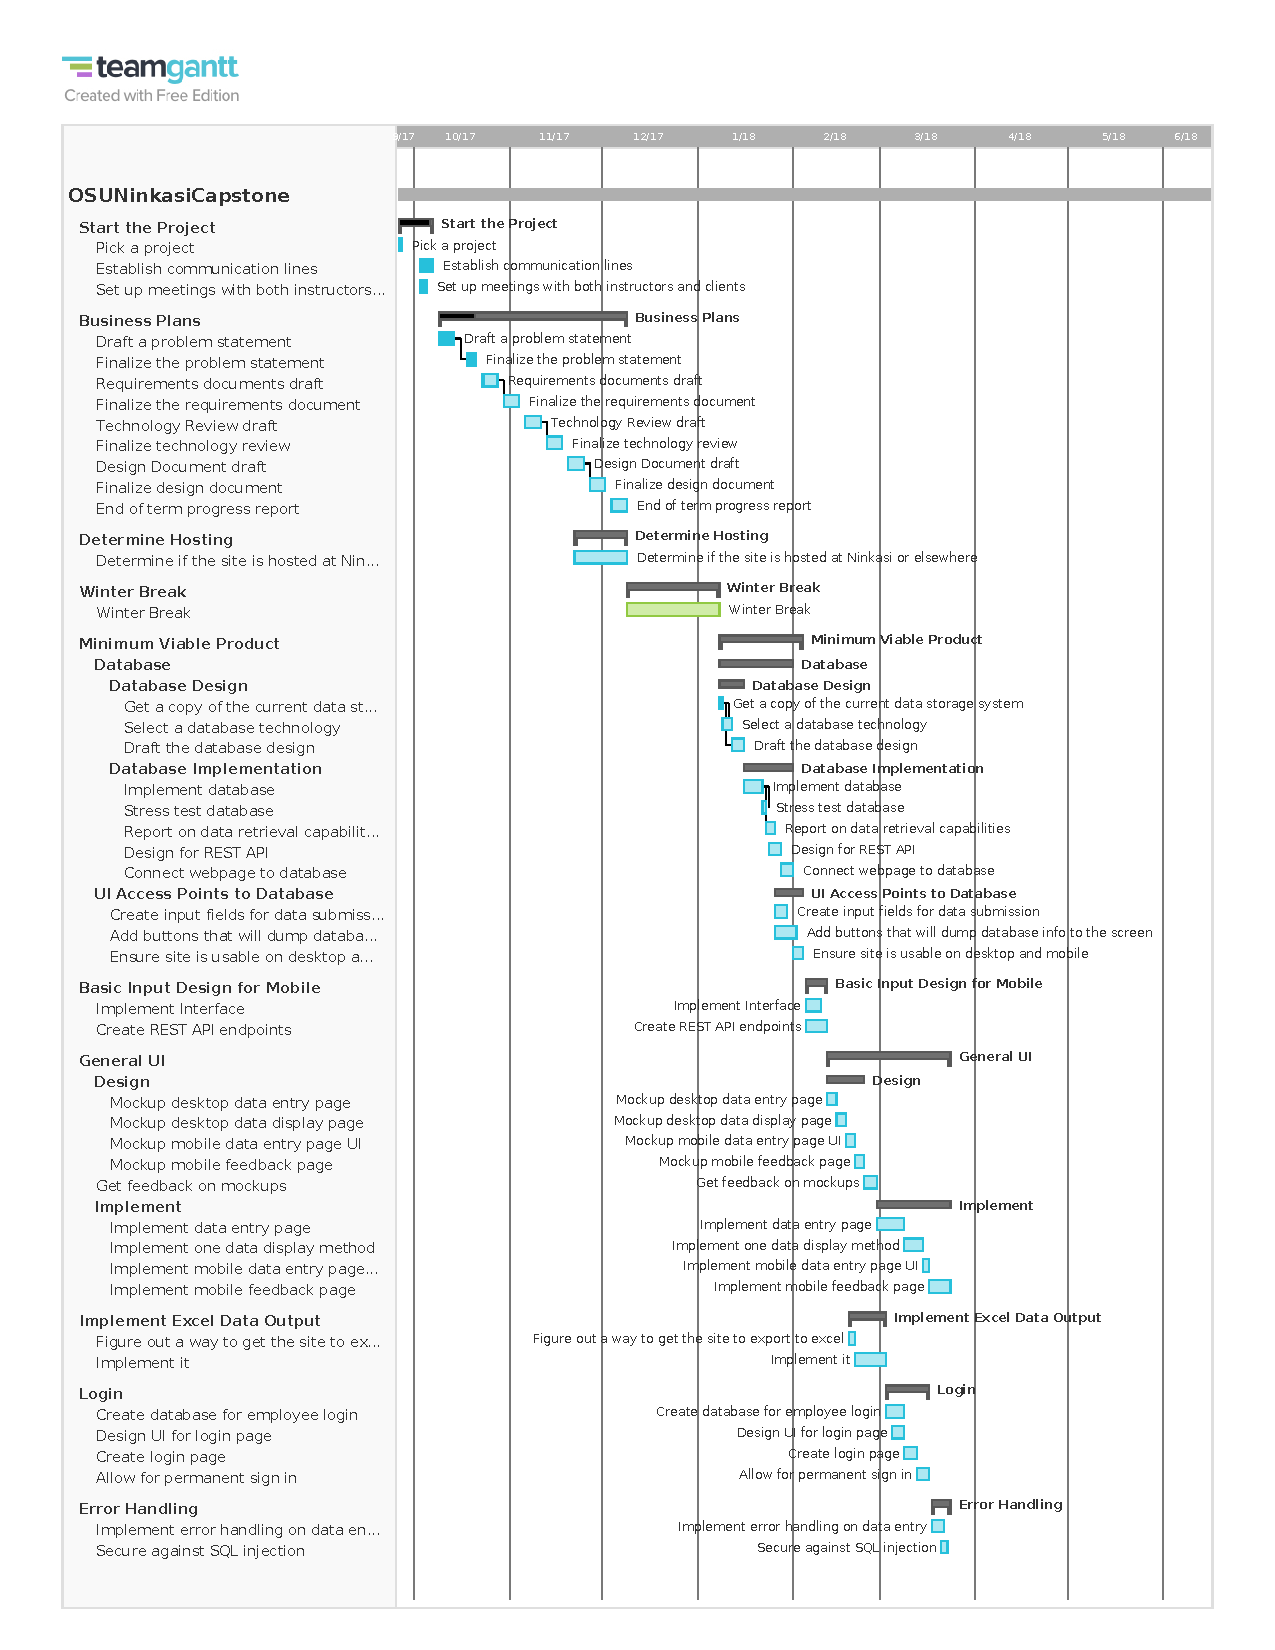
\includepdf[pages=1-2]{OSUNinkasiCapstone.pdf}

\end{document}
